\documentclass[titlepage]{article}
\title{The last project of workshop class}
\author{Sina Fallahi}
\usepackage{xcolor}
\usepackage{graphicx}
\graphicspath{ {./images/} }
\usepackage{fancyhdr}

\setlength{\headheight}{15pt}
\pagestyle{fancy}
\fancyhf{}
\rhead{Sina Fallahi}
\lhead{Final project of workshop}
\rfoot{Page \thepage}
\begin{document}

\maketitle
\section{intro}
hello i'm sina fallahi. I have just written the first steps of this latex file

\section{Git and GitHub}

\subsection{Repository Initialization and Commits}
Write about how you set up the repository for this assignment. Explain every step in
detail.\\
the answer: \textcolor{blue}{first I made a repository in Github and after that i cloned it to my local machine then I added the workflow folder and a latex file for testing after that I used tags for pushing my latex file: git tag [tag name] + git push [tag name]}
\\ \\Provide a walkthrough of setting up GitHub Actions to automatically compile your LaTeX
document and any challenges you encountered.\\
the answer: \textcolor{blue}{for compiling the latex file I had a challenge and I fixed It by giving the permission of read and write to the actions in the setting}
\section{exploration tasks}
\subsection{Vim Advanced Features}
Explore and document 3 advanced features of Vim that were not covered in class.\\answer: \textcolor{blue}{the command :verbose will output at what line of what file a precise configuration have been declared.\\ gf edits the file located at the file path under my cursor.\\ CTRL+W CTRL+F wil open the file in a new window.}
\subsection{Memory profiling}
This semester, you got to know about dynamic memory allocation in C in your Programming Fundamentals class.
\subsubsection{Memory leak}
This semester, you got to know about dynamic memory allocation in C in your Programming Fundamentals class.\\ answer: 
\textcolor{blue}{Memory leak happen when a memory that is allocated for a particular purpose in not properly deallocated or released when it is no longer needed , leading to a gradual loss of available memory over time}
\subsubsection{memory profilers}
Read about a tool called Valgrind and write about their purpose and how it helps when
memory leaks happen.
\\answer: \textcolor{blue}{Valgrind is an open source programming tool suite that provides a collection of tools for debugging a collection of tools for debugging and profiling Linux and Unix programs and its primary purpose is to detect Various memory related errors in programs such am memory leaks buffer overflows and invalid memory accesses in memory leaks it identifies blocks of dynamically allocated memory that are not properly deallocated, leading to memory leaks and potential resource exhaustion.}
\subsection{GNU/Linux Bash Scripting}
\subsubsection{fzf}
What is fuzzy searching? Give a short description.\\answer: \textcolor{blue}{fuzzy searching is a way that when we dont have a complete idea of what we are looking for we can use.\\}
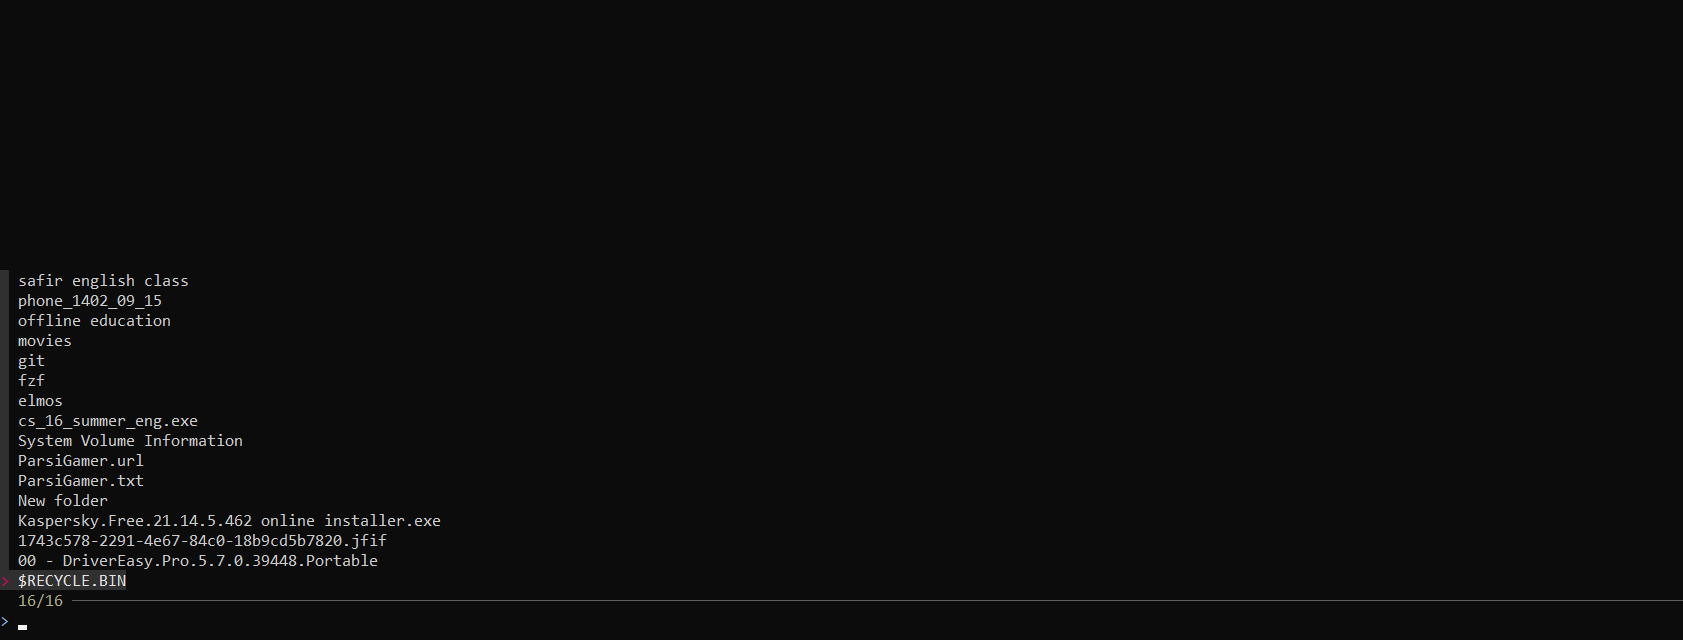
\includegraphics[width = 1.2\textwidth]{fzf0}
\newpage the image:
\subsubsection{Using fzf to find your favorite PDF}
\textcolor{blue}{we can use fdfind .pdf | fzf as shown in} 
\begin{figure}[h]
\centering
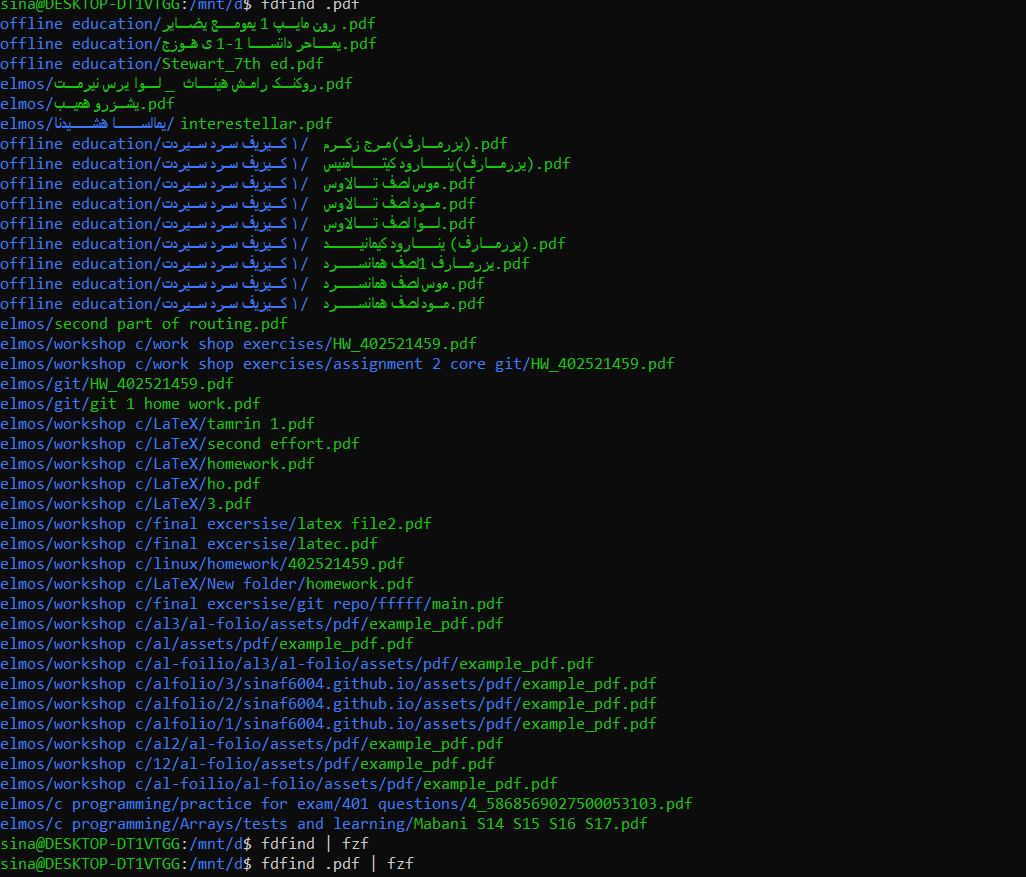
\includegraphics[width = 1.2\textwidth]{fzf2}
\end {figure}
\newpage
\section{Opening the file using Zathura}
after installing the package of zathure we can give the path and open the file\\
\textcolor{blue}{we can use fdfind .pdf | fzf as shown in} 
\begin{figure}[h]
\centering
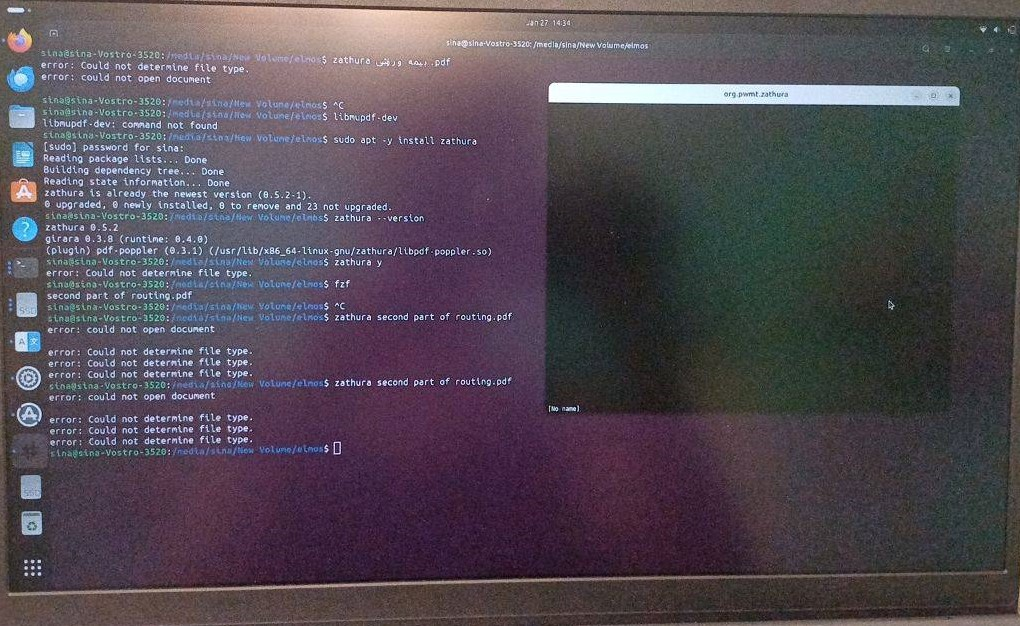
\includegraphics[width = 1.2\textwidth]{ssss}
\end {figure}
but the only problem of this picture is that the name of the files must get seperated by $\backslash$ and because of that It could not open the pdf.
\section{read me}
\textcolor{blue}{the read m file added}
\newpage
\section{issue}
\textcolor{blue}{the issue is available in your repository
this is the screen shot:}
\begin{figure}[h]
\centering
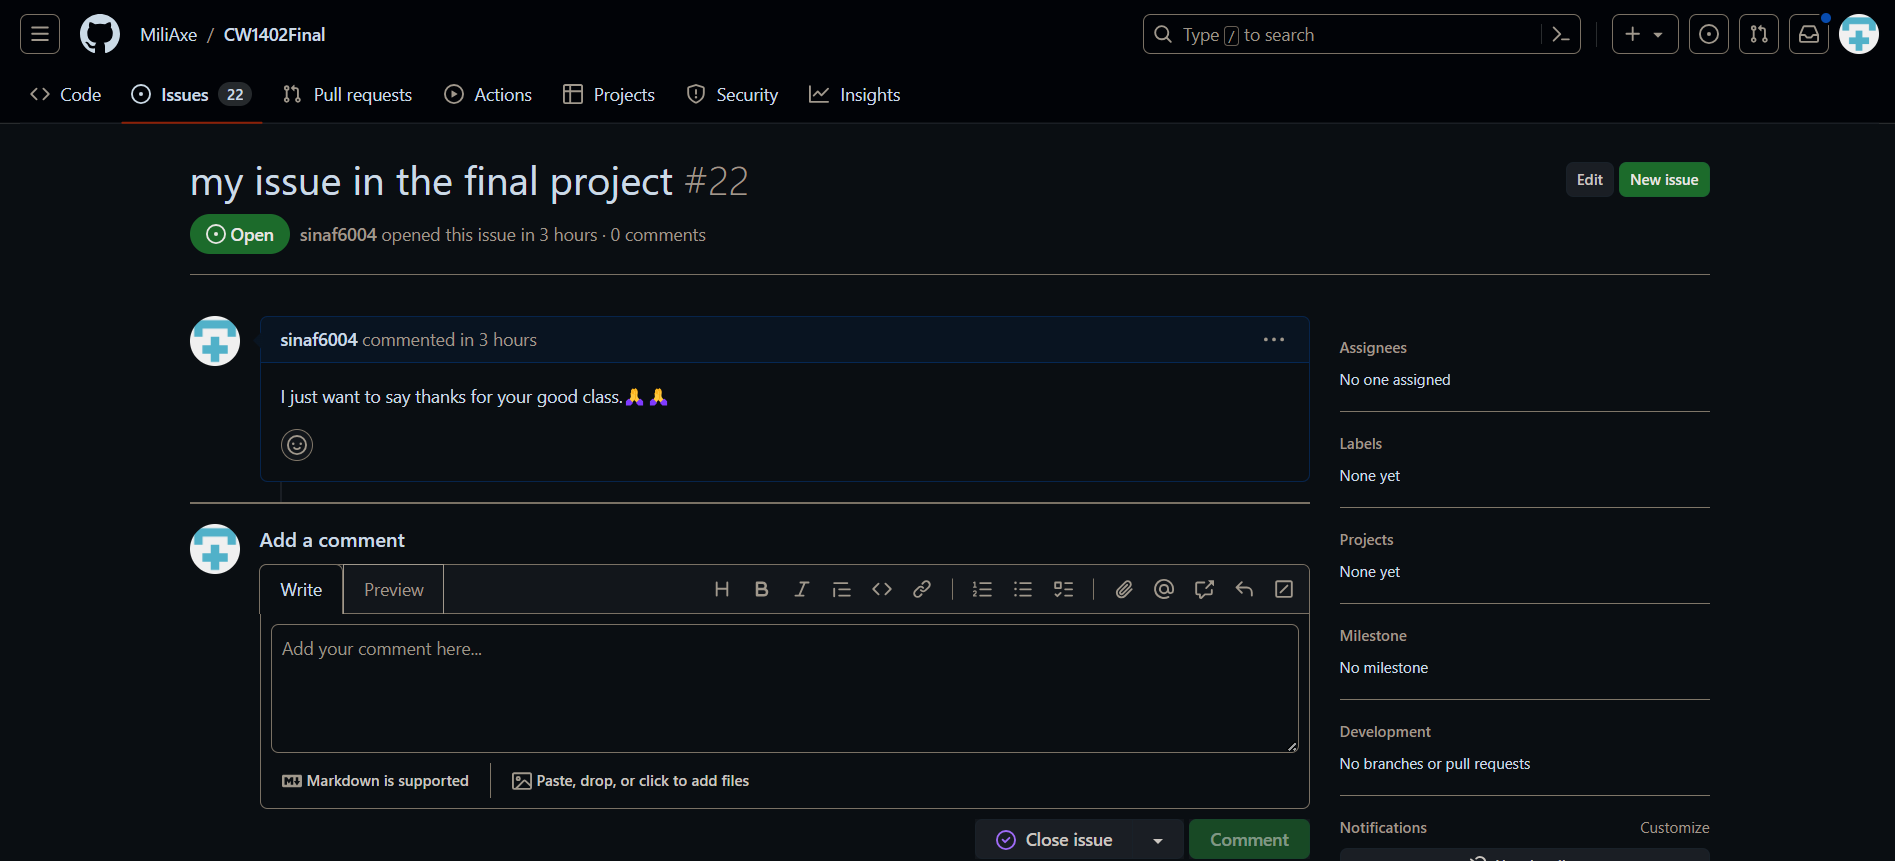
\includegraphics[width = 1.2\textwidth]{issue}
\end {figure}
\\\\\\\\\\the repository link: https://github.com/sinaf6004/fffff
\\student number = 402521459


\end{document}

